\chapter{Experiments}
\label{sec:chapter5}
In the previous chapter, the method for Human Activity Recognition by \cite{luvizon_2d/3d_2018} was introduced by explaining the model architectures and the Soft-argmax function proposed in \cite{luvizon_human_2017}.
Afterwards, this thesis proposed experiments to gain a better insight into the authors method by evaluating the model for different hyperparameters, as well as to investigate whether end-to-end training is feasible.
First, this chapter introduces the datasets in Section \ref{sec:exp-datasets}, which consist of the \textit{MPII Human Pose} dataset for $2D$ pose estimation and the \textit{Penn Action} and \textit{JHMDB} datasets for Human Activity Recognition.
Second, the metrics used in the authors work, as well as the experiments done in this thesis, are discussed in Section \ref{sec:exp-metrics}.
Third, this chapter discusses the experiment setups, as well as the results, in Section \ref{sec:exp-results}.
The pose estimation and $2D$ HAR experiments from \cite{luvizon_2d/3d_2018} are recreated first.
Further experimentation towards understanding the capabilities of the model are presented, including a qualitative and quantitative evaluation of the Soft-argmax function, the accuracy of the authors model achieved on the complex JHMDB dataset, as well as an approach for training the model in an end-to-end approach, without using a pretrained pose estimator.

\section{Datasets}
\label{sec:exp-datasets}
In the following section, three datasets are introduced.
The MPII Human Pose and Penn Action datasets are used to recreate the authors work.
The JHMDB dataset, which contains video clips with pose annotations for each frame, is used to evaluate how the model proposed in \cite{luvizon_2d/3d_2018} adapts to a more challenging video dataset.

\subsection{MPII Human Pose}
\label{sec:exp-mpii}

In \cite{andriluka_2d_2014}, the authors present a dataset for estimating two dimensional human pose on image data.
It contains pose annotations for $40.000$ persons in $25.000$ images.
The annotations include $16$ joint positions and an indicator of whether or not the joint is occluded or not.
The $16$ joints are \textit{left / right ankle}, \textit{left / right knee}, \textit{left / right hip}, \textit{left / right elbow}, \textit{left / right shoulder}, \textit{left / right wrist}, \textit{pelvis}, \textit{thorax}, \textit{upper neck} and \textit{top of the head}.
See \fref{fig:mpii_example_images} for example images of the dataset.
In addition, the body center coordinates, as well a scale indicating the size of the person bounding box are given by the dataset.
The scale is given with regards to a $200$ pixel bounding box, meaning that the bounding box side lengths can be computed by multiplying the scale with $200$.
Also, a bounding box of the head is given, which is used to compute the \textit{PCKh} metric (see \sref{sec:exp-pckh}).
The images are extracted from YouTube videos and they do not contain artifacts commonly found in videos, e.g., compression or blur.
Additionally, each image is assigned with an activity, totalling $401$ activities.
However, these annotations are not used for Human Action Recognition since the number of samples per activity is too low for training a model as complex as the HAR pipeline presented in \sref{sec:deephar_approach}.

\begin{figure}[htb!]
    \centering
    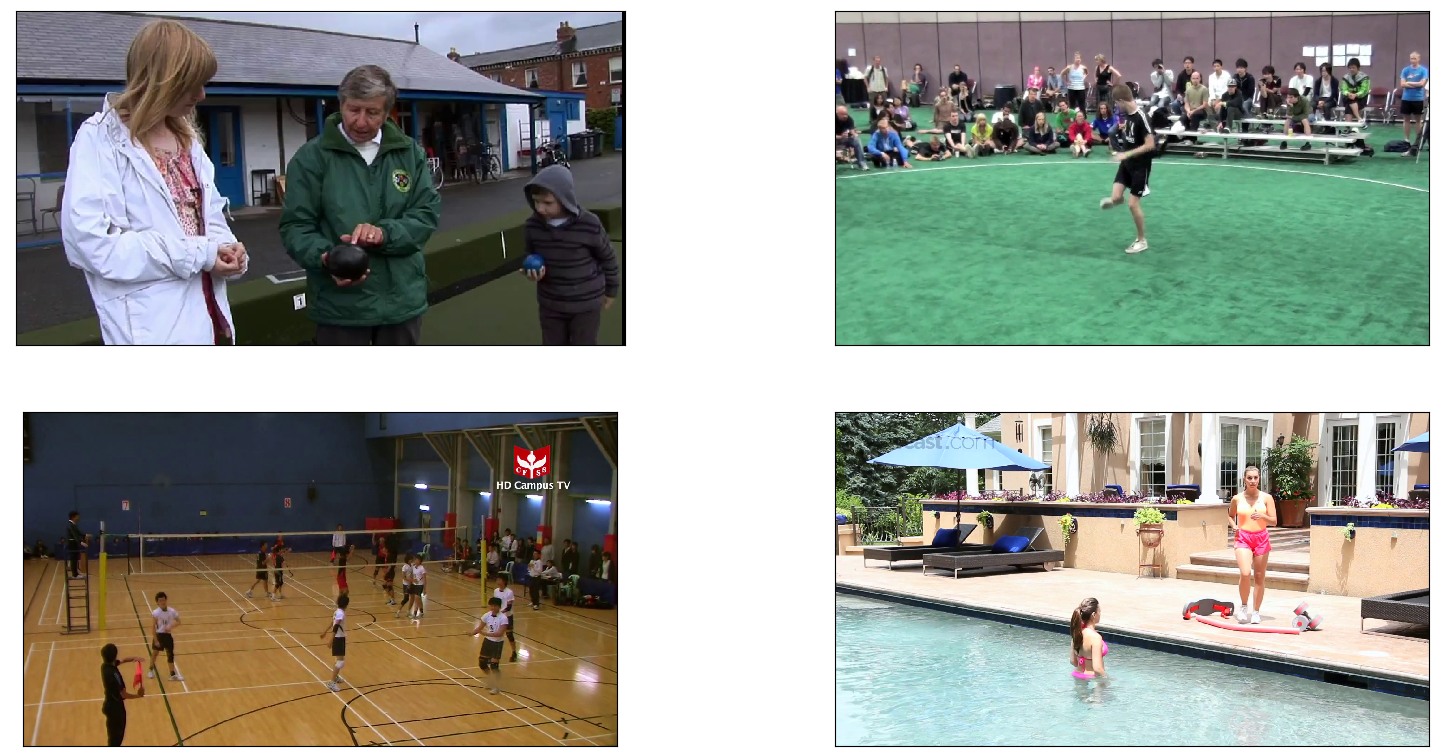
\includegraphics[width=0.7\textwidth]{mpii_example_images.png}
    \caption{Four example images from the MPII dataset \cite{andriluka_2d_2014}. }
    \label{fig:mpii_example_images}
\end{figure}

We follow the approaches from \cite{luvizon_2d/3d_2018} for preprocessing.
First, a person bounding box is estimated using the center body annotation from the dataset.
The authors multiply the scale given by the annotation $s_{orig}$ by $1.25$, resulting in $s_{new}$.
They do not motivate the reason for using this specific value, but it most likely was used to enlarge the bounding box to contain more context around the person.
Next, they compute the width and height using $s_{new} \cdot 200$, since the scale parameter in the dataset is given w.r.t. a $200 \times 200$ pixel bounding box.
In addition, the authors also alter the center position $(c_x,  c_y)$ by computing $(c_{x}^{new}, c_y^{new}) = (c_x, c_y + s_{new} \cdot 12)$.
Again, the authors do not provide a reasoning for increasing the center $y$ position.
Once the bounding box is computed, the image is cropped to the size of the bounding box around the newly computed center coordinate and rescalled to a size of $256 \times 256$.
In the case where a joint annotation falls outside of the now cropped image, the authors set the visibility of the joint to $0$ and set the $(x,y)$ coordinates of the joint to $(-1e9, -1e9)$.

Additionally, the authors introduce parameters used for image augmentation by rotating, scaling and mirroring the image randomly.
These values are sampled from their respective sets whenever augmentation is performed.
Specifically, they introduce $s_{aug} \in \{0.7, 1, 1.3\}$, which gets multiplied with $s_{new}$ computed earlier.
This results in zooming into or out of the image by $30\%$ when $s_{aug} \not= 1$. 
Also, $r_{aug} \in \{-40, -35, \dots, 35, 40\}$ is introduced to rotate the image $r_{aug}$ degrees around its center, possibly introducing black borders around the image.
Moreover, when augmenting, the image is horizontally mirrored with a chance of $50$ percent.
See \fref{fig:mpii_example_augmentation} for examples of different augmented images, including augmented pose.

\begin{figure}[htb!]
    \centering
    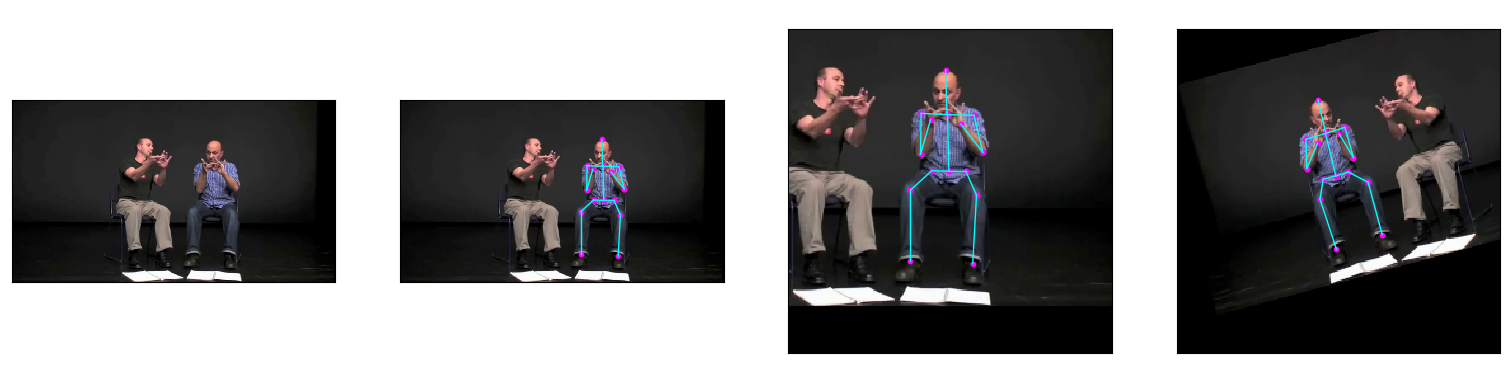
\includegraphics[width=0.99\textwidth]{mpii_dataset_augmented_examples.png}
    \caption{\textbf{From left to right}: \textbf{1.} Original image from the MPII dataset. \textbf{2.} Original image with the ground truth pose superimposed. \textbf{3.} Image after estimating the bounding box, cropping and rescaling. \textbf{4.} Augmented image using $s_{aug} = 1.3$, $r_{aug} = -15$ degrees and flipping the image horizontally.}
    \label{fig:mpii_example_augmentation}
\end{figure}

% When using horizontal mirroring, a problem occured where the estimated poses resembled a generic skeleton.
% See \fref{fig:ghost_skeleton} for an example image.
% Because of the horizontal flipping of the image, the pose needed to be flipped as well.
% Furthermore, however, the labels of some joints needed to be changed as well.
% As an example, the right arm (from the perspective of the subject in the image) becomes the left arm when the image is flipped.

% \begin{figure}[htb!]
%     \centering
%     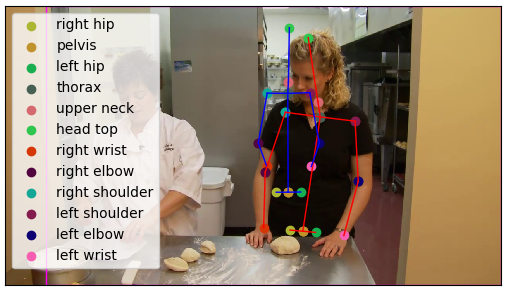
\includegraphics[width=0.80\textwidth]{ghost_skeleton.png}
%     \caption{Example of a phenomenon which occured when the image and pose were flipped durring augmentation, but the annotations were not properly changed. As an example, the left arm becomes the right arm after flipping. The ground truth pose is shown in red, while the learned pose is shown in blue. }
%     \label{fig:ghost_skeleton}
% \end{figure}

The dataset does not contain annotations for the test data, other than the scale and center coordinates.
To evaluate the test images, the joints need to be evaluated and the results need to be send to the authors of the dataset at the \textit{Max Planck Institute for Intelligent Systems} for comparison to the ground truth pose.
This ensures that the test data annotations are not mistakenly or maliciously used in training.
For all datasets used in the experiments, $10$ percent of the training datapoints are withheld from training and used as validation data.

\subsection{Penn Action}
\label{sec:exp-penn}

Another dataset used in \cite{luvizon_2d/3d_2018} is the Penn Action dataset \cite{zhang_actemes_2013}.
It contains $2326$ video clips of $15$ different, resulting in $149.355$ frames.
The actions are mostly sports related and they include \textit{baseball swing}, \textit{clean and jerk}, \textit{jumping jacks}, \textit{pushup}, \textit{strum guitar}, \textit{bench press}, \textit{golf swing}, \textit{baseball pitch}, \textit{situp}, \textit{tennis forehand}, \textit{bowling}, \textit{jump rope}, \textit{pullup}, \textit{squat} and \textit{tennis serve}.
Additionally, the authors provide annotations for $13$ body joints,
including \textit{left and right shoulders, elbows, wrists, hips and knees} and \textit{head}.
Some example images can be seen in \fref{fig:pennaction_example_images}. 

\begin{figure}[htb!]
    \centering
    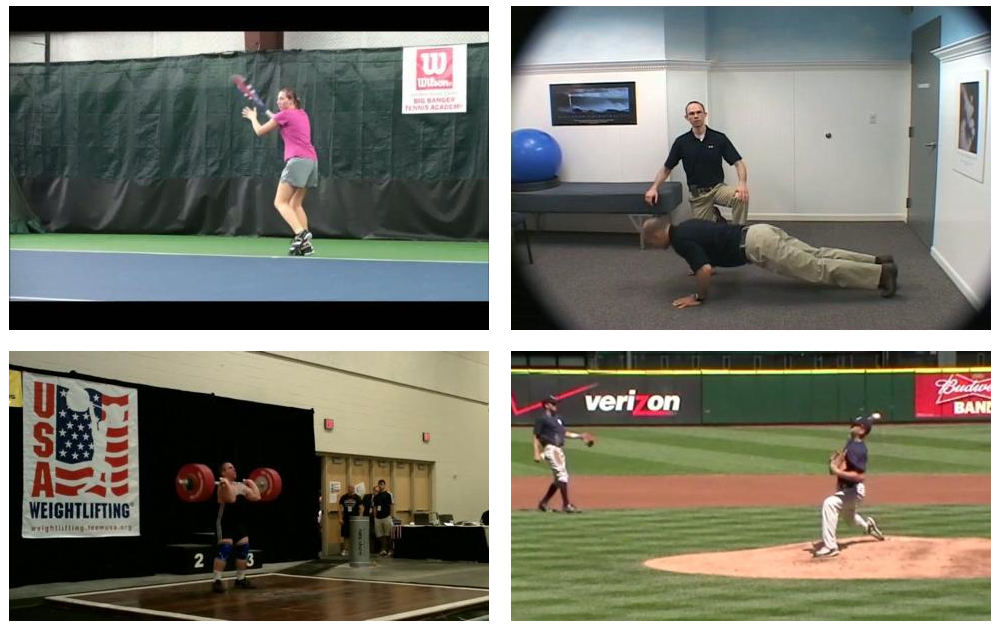
\includegraphics[width=0.7\textwidth]{pennaction_example_images.png}
    \caption{Four example images from the Penn Action dataset \cite{zhang_actemes_2013}. }
    \label{fig:pennaction_example_images}
\end{figure}

It was decided by \cite{luvizon_2d/3d_2018} that the number of joints should be identical to the ones presented in \cite{andriluka_2d_2014} \sref{sec:exp-mpii}.
This is important, because the network architecture is designed in a way that assumes $16$ joints per video frame because the estimated poses for each frame of a video clip are aggregated in a fixed size \textit{pose cube} representation (see \sref{sec:pose_based_action_recognition}).
To achieve this, the \textit{head} annotation of the Penn Action dataset is mapped to the \textit{upper neck} joint of the MPII dataset and the missing joints were interpreted as not visible.

Additional augmentation is introduced to make the training process more robust.
Two additional augmentation methods are used.
First, salt and pepper augmentation is applied to the training images with a probability of $0.5$.
In this augmentation method, each pixel is set to either black or white with probability $p_{sp} = 0.02$.
Second, black rectangles are placed randomly inside the image, occluding parts of the original image.
The network needs to make decisions on partially occluded images, making it more robust, because it forces the network to utilize alternative paths on some images, effectively making the model more general.
Dropout is applied with a probability of $0.5$ as well.

For some experiments, ground truth bounding boxes of the person are calculated by taking the minimum and maximum of the $x$ and $y$ coordinates from the ground truth pose and defining these as the corners of the bounding box.
Additionally, to include more context around the person, the bounding box is increased in both dimensions.
This was done to add more context around the subject, but also because the Soft-argmax function is unprecise around the image borders (see \sref{sec:exp-softargmax-accuracy}).
For high uncertainty of the pose location, the Soft-argmax function is unprecise for approximately $20$ pixels around the image border (see \fref{fig:deeppose-qualitative}).
Thus, the amount of context added is set to $30$ pixels to make certain that the Soft-argmax function does not wrongly estimates the pose position.

Additionally, the authors in \cite{luvizon_2d/3d_2018} decide to process the video clips in chunks of $16$ frames.
This is important since the network architecture assumes a specific dimensionality for the \textit{pose cube} (see \sref{sec:pose_based_action_recognition}).
These chunks are further referred to as \textit{fragments}. 

\subsection{JHMDB}
\label{sec:exp-jhmdb}

Similar to \cite{zhang_actemes_2013} \sref{sec:exp-penn}, the JHMDB dataset \cite{jhuang_towards_2013} contains annotations for the pose and the action in video clips.
The dataset was created by taking a subset of the HMDB action recogntion dataset \cite{kuehne_hmdb:_2011}, which was annotated using the \textit{puppet tool} \cite{zuffi_pictorial_2012}.
This tool allows to not only annotate the pose of the person but also automatically computes a binary segmentation map of the person, further referred to as the \textit{puppet mask}.
See \fref{fig:puppet_tool_example} for a visualization of the annotation process and the puppet tool.

\begin{figure}[htb!]
    \centering
    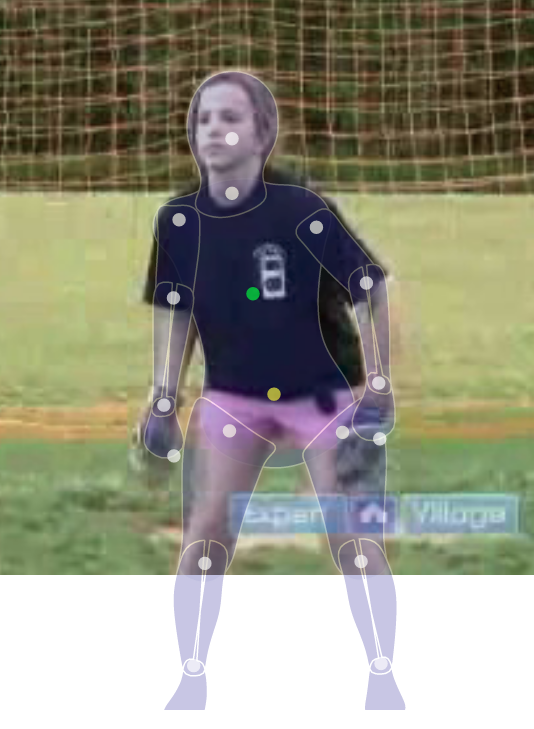
\includegraphics[width=0.4\textwidth]{puppet_tool_example.png}
    \caption{Example of an image, annotated using the puppet flow. The dots indicate the joint positions, while the transparent human figure prior automatically adjusts, yielding the human segmentation map. Notice that, by using the figure, even joints that are not visible (like the ankles) still get anatomically plausible annotations. Image taken from \cite{max_planck_institute_for_intelligent_systems_jhmdb_nodate}.}
    \label{fig:puppet_tool_example}
\end{figure}

The clips in the HMDB dataset are taken from YouTube.
The annotated subset contains the following actions:
\textit{brush hair}, \textit{catch}, \textit{clap}, \textit{climb stair}, \textit{golf}, \textit{jump}, \textit{kick ball}, \textit{pick}, \textit{pour}, \textit{pullup}, \textit{push}, \textit{run}, \textit{shoot ball}, \textit{shoot bow}, \textit{shoot gun}, \textit{sit}, \textit{stand}, \textit{swing baseball}, \textit{throw}, \textit{walk} and \textit{wave}.
Some example images of the dataset can be seen in \fref{fig:jhmdb_example_images}.
Notice that the actions are more diverse, in comparison to the Penn Action dataset, specifically because it also contains non-sport activities.

\begin{figure}[htb!]
    \centering
    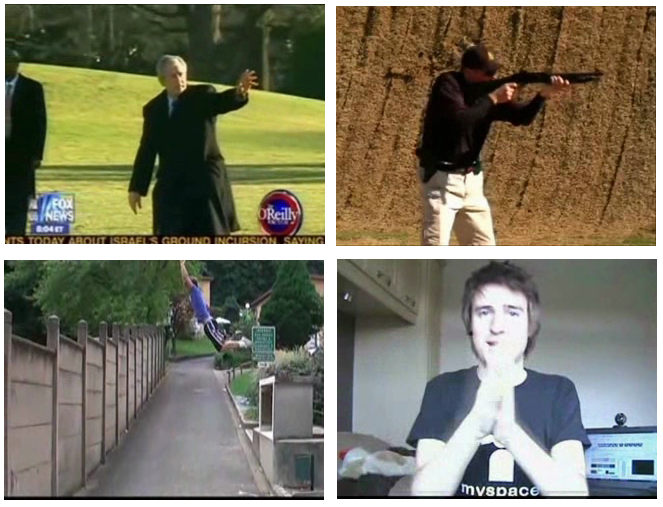
\includegraphics[width=0.7\textwidth]{jhmdb_example_images.png}
    \caption{Four example images from the JHMDB dataset \cite{jhuang_towards_2013}. }
    \label{fig:jhmdb_example_images}
\end{figure}

The puppet tool defines $15$ different joints.
They are identical to the ones annotated in the Penn Action dataset, but they additionally contain the \textit{neck} and the \textit{belly}.
Also, the approaches for computing ground truth bounding boxes, preprocessing and augmenting the \textit{fragments} are identical to the ones presented earlier in \sref{sec:exp-penn}.

\section{Evaluation Metrics}
\label{sec:exp-metrics}
In this section, the \textit{PCK} and \textit{PCKh} metrics are presented, which are used to evaluate the accuracy of the predicted pose in comparison to the ground truth annotation.
Also, two approaches for assessing the accuracy in video clips, \textit{Single-} and \textit{Multi-Clip accuracy}, are presented.

\subsection{PCK}
\label{sec:exp-pck}

The \textit{Probability of Correct Keypoints (PCK)} metric \cite{ferrari_progressive_2008} is often used in the literature to evaluate an estimated pose when a human bounding box is given.
See \sref{sec:pck_related_work} for a motivation of this metric.
Let $k_{est} = (x_{est}, y_{est})$ be a predicted joint location and let $k_{gt} = (x_{gt}, y_{gt})$ be the corresponding ground truth joint location.
First, the absolute distance $d = \lVert k_{est} - k_{gt} \rVert$ is computed.
Second, the maximum of the bounding box side lengths $l_{max} = max(bbox_{height}, bbox_{width})$ is computed and multiplied by a hyperparameter $\alpha$, resulting in $l_{comp} = l_{max} \cdot \alpha$.
Then, an estimated joint location is determined to be estimated correctly if $d < l_{comp}$.
The hyperparameter $\alpha$ is a threshold, which determines how close the predicted joint location has to be to the ground truth joint location in order to be classified as correctly estimated.
Typical values for $\alpha$ found in the literature are $0.2$ and $0.1$.
This metric is used primarily for evaluating the pose on the JHMDB dataset since the dataset does not provide head bounding box annotations, which are necessary for using the PCKh metric.

To compensate for the lack of head annotation, this thesis proposes to use an additional metric for evaluating predicted poses, referred to as \textit{PCKu}.
Instead of using the bounding box side lengths to determine $l_{comp}$, the distance between the neck joint position and pelvis joint position is used.
While this is not as invariant to different actions and poses as PCKh, it is more robust in comparison to traditional PCK.
This metric is computed in addition to PCK for datasets which do not provide a head bounding box annotation.

\subsection{PCKh}
\label{sec:exp-pckh}
One downside of using the PCK metric based on person bounding box side lengths is that poses where one or more limbs are stretched out far from the subjects torso the bounding box is not an accurate representation of the body size.
Thus, the threshold $l_{comp}$ highly depends on the pose of the person, which can lead to a higher threshold, depending on the action.
Consider the difference in subject bounding box size between a person sitting on a chair versus a person jumping in the air while spreading their arms.

In \cite{andriluka_2d_2014}, the authors propose the head bounding box diameter, assuming that this bounding box does not change for different poses.
See \sref{sec:pose-machine-evaluation} for a motivation of the metric.
Similar to PCK, PCKh also defines a threshold parameter $\alpha$.
Typical values for $\alpha$ found in the literature are $0.5$ and $0.2$.

\subsection{Single- and Multi-Clip Accuracy}
To evaluate the accuracy of the HAR pipeline, the authors in \cite{luvizon_2d/3d_2018} use two different approaches.
First, they take the video to evaluate and extract a $16$ frame long clip from the middle of the video.
Second, they classify the action of that $16$ frame clip.
Since the output of the network is a Softmax activation, they use the \textit{argmax} function to determine the action with the highest score.
This is referred to further as \textit{Single-Clip accuracy}.

Additionally, the authors first extract multiple $16$ frame long clips from the video by starting at frame $0$ and then incrementing the starting position by $8$ for as long as there are at least $16$ frames left in the clip.
They do not motivate their choice of incrementing the starting position by $8$.
Second, for each clip, they predict the action.
Third, they determine the class most often predicted for the set of clips, which is then used to compare to the ground truth class of the video.
For example, if $4$ clips are extracted from the video using the method presented above, and $3$ of these clips are classified as \textit{shooting bow}, then \textit{shooting bow} is used for comparison to the ground truth action of the video.
The accuracy of this method is referred to as \textit{Multi-Clip accuracy}.

\section{Experimental Results}
% TODO: Think about if the network was actually overfitting everytime you write it. Hard to say without train accuracy. On the other hand, who will know...
% TODO: Einleitung schreiben
\label{sec:exp-results}
\subsection{Accuracy of Soft-argmax function}
\label{sec:exp-softargmax-accuracy}
In \cite{luvizon_human_2017}, the authors propose a method for finding pixel coordinates of the maximum pixel value in an image, which they refer to as \textit{Soft-argmax} (see \sref{sec:softargmax}).
They argue that this method can be used instead of the Argmax function, which is often used for the same purpose.
This suggests that the Soft-argmax should be as accurate in determining the maximum values as the Argmax function.
To investigate this assumption, this thesis performs two experiments.
% For both experiments, an estimated coordinate $(x_{est},y_{est})$ is considered to be correct in comparison to the ground truth coordinate $(x_{gt}, y_{gt})$ if both $\lvert x_{est} - x_{gt} \rvert \leq d$ and $\lvert y_{est} - y_{gt} \rvert \leq d$.
% The reason for using a threshold of $d$ pixels is that the output of the Soft-argmax function are fractions of width and height with $(x_{frac}, y_{frac}) \in [0,1]$.
% To compute the image coordinates, a multiplication with the width and height of the input image is necessary.
% Also, the resulting floating point values need to be rounded to the nearest integer in order to be considered image coordinates.
% Because the rounding process might introduce errors, a threshold of $d$ is defined.
% By varying $d$, the accuracy of the Soft-argmax can be determined. 

In the first experiment, we analyze the accuracy quantitatively on data from the MPII dataset.
For each joint position $(i,j)$ of a pose, a synthetic joint heatmap is generated by placing a two-dimensional gaussian with mean $(i,j)$ and covariance $c$.
The Soft-argmax is applied to the heatmap, which results in estimates $(x_{est},y_{est})$ of the maximum.
The distance from $(x_{est},y_{est})$ to $(i,j)$ is computed and an accuracy meassurement is proposed by the following formula:

\begin{equation}
    f((x_{est}, y_{est}), (i,j), d) = 
    \begin{cases}
        1 & \text{if} ~ \lvert x_{est} - i \rvert \leq d ~ \text{and} ~ \lvert y_{est} - j \rvert \leq d \\
        0 & \text{otherwise}
    \end{cases}
    \label{eq:acc_softargmax}
\end{equation}

In \eref{eq:acc_softargmax}, $d$ refers to a threshold, which is necessary because of the way $(x_{est}, y_{est})$ is computed.
The output of the Soft-argmax function are fractions of width and height with $(x_{frac}, y_{frac}) \in [0,1]$.
These fractions need to be multiplied by the width and height and they need to be rounded to the nearest integer afterwards to get valid image coordinates.
This rounding process might introduce rounding errors.
This thesis evaluates the accuracy of the Soft-argmax for different values of $d$ on a subset of $1000$ random images from the MPII dataset.
Moreover, different covariance values $c \in \{1, 2, 5, 10, 20, 50 \}$ are used to simulate different uncertainties in the heatmap.
The results can be seen in \tref{tab:softargmax_numeric_eval}.

As can be seen in \tref{tab:softargmax_numeric_eval}, the Soft-argmax function is accurate in practice for a $2$ pixel threshold.
For higher values of $c$, the Soft-argmax becomes less accurate.
This is to be expected, given that the heatmap is less certain of the true pixel coordinate.
Notice that the accuracies are significantly lower for a threshold of $d=1$.
This contrast between $d=1$ and $d=2$ is most likely due to the rounding errors discussed earlier.

\begin{table}[]
    \centering
    \scalebox{0.90}{%
    \begin{tabular}{|l|l|l|l|l|l|l|}
    \hline
    threshold & \textbf{$c=1$} & \textbf{$c=2$} & \textbf{$c=5$} & \textbf{$c=10$} & \textbf{$c=20$} & \textbf{$c=50$} \\ \hline
    $1$ & 93.137 & 93.123 & 93.069 & 92.988 & 92.811 & 92.201 \\ \hline 
    $2$ & 99.952 & 99.931 & 99.843 & 99.741 & 99.469 & 98.598 \\ \hline 
    $3$ & 99.959 & 99.945 & 99.891 & 99.809 & 99.639 & 99.054 \\ \hline 
    $4$ & 99.959 & 99.952 & 99.911 & 99.829 & 99.700 & 99.197 \\ \hline 
    \end{tabular}}
    \caption{Mean average accuracy (in percent) of Soft-argmax when detecting ground truth coordinates from synthetic joint heatmaps. Threshold referrs to the amound of pixels the estimate is allowed to deviate from the ground truth annotation. $c$ referres to the covariance used for creating the synthetic heatmaps. The large discrepancy between a threshold of $1$ and a threshold of $2$ is most likely due to rounding errors.}
    \label{tab:softargmax_numeric_eval}
\end{table}

In the second experiment, a synthetic image of size $255 \times 255$ pixels is created, since this is the size of the input images to the network after preprocessing.
For each $(i,j)$ position of the image, a two-dimensional gaussian with mean $(i,j)$ and covariance $c$ is placed.
Next, $(x_{est},y_{est})$ are computed using the Soft-argmax function.
Then, the estimations are compared to the ground truth mean value of the gaussian, i.e., $(i,j)$, using the accuracy function defined in \eref{eq:acc_softargmax} with $d=2$ to allow for a small rounding error.
This procedure is repeated for each $(i,j)$ coordinate of the image.
See \fref{fig:softargmax_variance_test} for a visualization of the results, where violett pixels indicate a wrong prediction and yellow pixels indicate a correct prediction.
As can be seen in the visualization, the Soft-argmax function accurately regresses the gaussian mean values for small covariances $c$ for most of the image coordinates.
As the covariance increases, the accuracy decreases, especially around the borders of the image.
While this behaviour indicates that the Soft-argmax function is less accurate around the borders of the image, this does not negatively effect the accuracy when estimating actual pose coordinates, according to the quantitative experiment.

\begin{figure}[htb!]
    \centering
    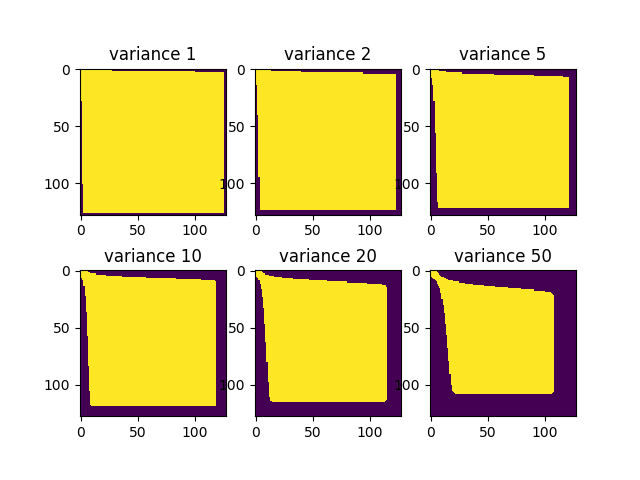
\includegraphics[width=0.7\textwidth]{softargmax_variance_test.png}
    \caption{Evaluation of the accuracy of the Soft-argmax function using synthetic data. Yellow pixels $(i,j)$ indicate where the Soft-argmax function correctly regressed the peak of the gaussian with mean value $(i,j)$, while violett indicates wrong predictions. Notice that the accuracy decreases when approaching the border of the image and when the covariance is increasing. }
    \label{fig:softargmax_variance_test}
\end{figure}

\subsection{Replication of Original Work}
\label{sec:exp-replication}
% TODO

First, to recreate the work of \cite{luvizon_2d/3d_2018}, a pose estimator using the MPII dataset is trained.
In addition to the authors work, the number of prediction blocks as well as the number of context heatmaps are varied to observe the effect on the overall accuracy of the model.
Second, the $2D$ HAR experiments, performed by the authors on the Penn Action datasets, are recreated.
The experiment settings are taken from \cite{luvizon_2d/3d_2018} as well as the supplemental material provided by the authors, if this thesis does not mention otherwise.

\subsubsection{Pose estimation}
\label{sec:exp-mpii-pose}
In \cite{luvizon_2d/3d_2018}, the authors use $8$ prediction blocks in their pose estimator (see \sref{sec:luvizon_poseestimator}) for evaluating the accuracy of the model on the MPII dataset, using the PCKh metric \sref{sec:exp-pckh}.
In this thesis, additional experiments using $2$ and $4$ prediction blocks are performed.
In addition, we evaluate all models without context heatmaps as well as with $2$ context heatmaps, to gain an insight into how using context maps effects the model performance.
From now on, this thesis uses the term \textit{model configuration} when refering to models with different number of prediction blocks and context heatmaps.

The training data of the MPII dataset is split into a training and validation set for evaluating the model's accuracy on unseen data.
An iteration is defined as the processing of one batch.
The batch size varies, depending on the experiment, since the models are of different size.
This means that, for smaller models, a bigger batch size is used since more data fits in GPU memory.
The batch size is set to $45, 30$ and $20$ for $2, 4$ and $8$ prediction blocks, respectively.
As an optimizer, the authors use the RMSProp algorithm.
An initial learning rate of $10^{-3}$ is used in accordance to the work of the authors.

\begin{equation}
    \label{eq:elasticnetloss}
    L_p = \frac{1}{N_j} \sum_{i=1}^{N_j} \lVert(p_{est} - p)\rVert_1 + \lVert p_{est} - p \rVert^2_2.
\end{equation}

The authors define a loss function named \textit{Elastic Net Loss}.
For each joint in the pose, the $L_1$ and $L_2$ norms between the estimated and ground truth joint are computed and added.
Then, these sums are again summed and normalized by the number of joints in the pose.
See \eref{eq:elasticnetloss}, where $p_{est}$ refers to the estimated joint position by the pose estimator and $p$ refers to the ground truth pose.
In addition to computing the Elastic net loss, the authors predict the visibility of each joint.
The annotations of MPII provide ground truth labels $v \in \{0,1\}$ of whether a joint is occluded or not.
The binary cross-entropy is used to compute a loss $L_v$ between the predicted visibility vector $v_{est}$ and the ground truth $v$.
Finally, both losses are combined in the following way:

\begin{equation}
    L = L_p + 0.01 \cdot L_v.
\end{equation}

For all subsequent pose estimation experiments, $L$ is used to compute the loss of the pose estimator.

As discussed before, for evaluating a model on the test dataset, the estimations need to be send to the \textit{Max Planck Institute for Intelligent Systems} for evaluation.
The amount of submissions is limit to $4$.
This means that it is not possible to evaluate all pose estimator configurations on the test dataset.
Thus, this thesis chooses to report the validation accuracy for comparison between the different model configurations and only submit estimations from the best performing model.

% \begin{table}[]
%     \small
%     \centering
%     \begin{tabular}{|l|l|c|c|}
%     \hline
%         \textbf{nr\_blocks} & \textbf{nr\_context}  & \textbf{PCKh @ 0.5} & \textbf{p-value} \\ \hline
%         \begin{tabular}{@{}c@{}} 2 \\ 2 \end{tabular} & \begin{tabular}{@{}c@{}} 0 \\ 2 \end{tabular} & \begin{tabular}{@{}c@{}} 84.15 \\ 84.01  \end{tabular} & 0.85  \\ \hline
    
%         \begin{tabular}{@{}c@{}} 4 \\ 4 \end{tabular} & \begin{tabular}{@{}c@{}} 0 \\ 2 \end{tabular} & \begin{tabular}{@{}c@{}} 85.78 \\ 85.64  \end{tabular} & 0.85  \\ \hline

%         \begin{tabular}{@{}c@{}} 8 \\ 8 \end{tabular} & \begin{tabular}{@{}c@{}} 0 \\ 2 \end{tabular} & \begin{tabular}{@{}c@{}} 86.71 \\ \textbf{87.00}  \end{tabular} & 0.73  \\ \hline

%         \begin{tabular}{@{}c@{}} 2 \\ 4 \end{tabular} & \begin{tabular}{@{}c@{}} 0 \\ 0 \end{tabular} & \begin{tabular}{@{}c@{}} 84.15 \\ 85.78  \end{tabular} & 0.074  \\ \hline

%         \begin{tabular}{@{}c@{}} 2 \\ 4 \end{tabular} & \begin{tabular}{@{}c@{}} 2 \\ 2 \end{tabular} & \begin{tabular}{@{}c@{}} 84.01 \\ 85.64  \end{tabular} & 0.076  \\ \hline

%         \begin{tabular}{@{}c@{}} 4 \\ 8 \end{tabular} & \begin{tabular}{@{}c@{}} 0 \\ 0 \end{tabular} & \begin{tabular}{@{}c@{}} 85.78 \\ 86.71  \end{tabular} & 0.31  \\ \hline

%         \begin{tabular}{@{}c@{}} 4 \\ 8 \end{tabular} & \begin{tabular}{@{}c@{}} 2 \\ 2 \end{tabular} & \begin{tabular}{@{}c@{}} 85.64 \\ \textbf{87.00}  \end{tabular} & 0.12  \\ \hline

%         \begin{tabular}{@{}c@{}} 2 \\ 8 \end{tabular} & \begin{tabular}{@{}c@{}} 0 \\ 0 \end{tabular} & \begin{tabular}{@{}c@{}} 84.15 \\ 86.71  \end{tabular} & \textbf{0.006}  \\ \hline

%         \begin{tabular}{@{}c@{}} 2 \\ 8 \end{tabular} & \begin{tabular}{@{}c@{}} 2 \\ 2 \end{tabular} & \begin{tabular}{@{}c@{}} 84.01 \\ \textbf{87.00}  \end{tabular} & \textbf{0.001}  \\ \hline
%     \end{tabular}
%     \caption{Different model configurations and their corresponding PCKh validation score. The $p$-values were computed using a randomization test. $p$-values below the significance level of $0.05$ are shown in bold, indicating that the change in accuracy is significant. Additionally, the highest accuracy is also shown in bold.} % TODO
%     \label{tab:mpii_results}
% \end{table}

\begin{table}[]
    \small
    \centering
    \begin{tabular}{ll}
        \begin{tabular}{|l|l|c|c|}
            \hline
            \textbf{blocks} & \textbf{context}  & \textbf{PCKh @ 0.5} & \textbf{p-values} \\ \hline
            \begin{tabular}{@{}c@{}} 2 \\ 2 \end{tabular} & \begin{tabular}{@{}c@{}} 0 \\ 2 \end{tabular} & \begin{tabular}{@{}c@{}} 84.15 \\ 84.01  \end{tabular} & 0.85  \\ \hline
        
            \begin{tabular}{@{}c@{}} 4 \\ 4 \end{tabular} & \begin{tabular}{@{}c@{}} 0 \\ 2 \end{tabular} & \begin{tabular}{@{}c@{}} 85.78 \\ 85.64  \end{tabular} & 0.85  \\ \hline
    
            \begin{tabular}{@{}c@{}} 8 \\ 8 \end{tabular} & \begin{tabular}{@{}c@{}} 0 \\ 2 \end{tabular} & \begin{tabular}{@{}c@{}} 86.71 \\ \textbf{87.00}  \end{tabular} & 0.73  \\ \hline
    
            \begin{tabular}{@{}c@{}} 2 \\ 4 \end{tabular} & \begin{tabular}{@{}c@{}} 0 \\ 0 \end{tabular} & \begin{tabular}{@{}c@{}} 84.15 \\ 85.78  \end{tabular} & 0.074  \\ \hline

            \begin{tabular}{@{}c@{}} 2 \\ 4 \end{tabular} & \begin{tabular}{@{}c@{}} 2 \\ 2 \end{tabular} & \begin{tabular}{@{}c@{}} 84.01 \\ 85.64  \end{tabular} & 0.076  \\ \hline

        \end{tabular}
        \begin{tabular}{|l|l|c|c|}
            \hline
            \textbf{blocks} & \textbf{context}  & \textbf{PCKh @ 0.5} & \textbf{p-values} \\ \hline
    
            \begin{tabular}{@{}c@{}} 4 \\ 8 \end{tabular} & \begin{tabular}{@{}c@{}} 0 \\ 0 \end{tabular} & \begin{tabular}{@{}c@{}} 85.78 \\ 86.71  \end{tabular} & 0.31  \\ \hline
    
            \begin{tabular}{@{}c@{}} 4 \\ 8 \end{tabular} & \begin{tabular}{@{}c@{}} 2 \\ 2 \end{tabular} & \begin{tabular}{@{}c@{}} 85.64 \\ \textbf{87.00}  \end{tabular} & 0.12  \\ \hline
    
            \begin{tabular}{@{}c@{}} 2 \\ 8 \end{tabular} & \begin{tabular}{@{}c@{}} 0 \\ 0 \end{tabular} & \begin{tabular}{@{}c@{}} 84.15 \\ 86.71  \end{tabular} & \textbf{0.006}  \\ \hline

            \begin{tabular}{@{}c@{}} 2 \\ 8 \end{tabular} & \begin{tabular}{@{}c@{}} 2 \\ 2 \end{tabular} & \begin{tabular}{@{}c@{}} 84.01 \\ \textbf{87.00}  \end{tabular} & \textbf{0.001}  \\ \hline
        
            \begin{tabular}{@{}c@{}} 8 \\ 8* \end{tabular} & \begin{tabular}{@{}c@{}} 2 \\ 2* \end{tabular} & \begin{tabular}{@{}c@{}} 87.00 \\ 89.00*  \end{tabular} & \textbf{0.025}  \\ \hline
        \end{tabular}                      
    \end{tabular}
    \caption{Different model configurations and their corresponding PCKh validation score. The $p$-values were computed using a randomization test. $p$-values below the significance level of $0.05$ are shown in bold, indicating that the change in accuracy is significant. Additionally, the highest accuracy is also shown in bold. The configuration marked with a star is the model from \cite{luvizon_2d/3d_2018}} % TODO
    \label{tab:mpii_results}
\end{table}


The PCKh accuracies achieved on the validation dataset from the different model configurations are shown in \tref{tab:mpii_results}.
For comparison, the authors report a validation accuracy of $89\%$ for $8$ prediction blocks and $2$ context heatmaps. 
As can be seen in \tref{tab:mpii_results}, the higher the number of prediction blocks, the more accurate the model performs on the validation data.
In addition, using context heatmaps appears to increase the accuracy only when using $8$ blocks.
To test whether or not the differences in accuracy between the configurations are statistically significant, this thesis performs randomization tests with a significance level of $0.05$.
For the randomization tests, $3000$ permutations are used.
As can be seen in \tref{tab:mpii_results}, the only statistically significant increases in accuracy are observed when comparing $2$ and $8$ prediction block models with and without context heatmaps.
This suggests that a certain depth of network is necessary in order for context heatmaps to contribute significantly to the model performance.
 
\begin{table}[]
    \centering
    \scalebox{0.90}{%
    \begin{tabular}{|l|l|l|l|l|l|l|l|l|c|}
        \hline
        &Head & Shoulder & Elbow & Wrist & Hip & Knee  & Ankle & Total & p-value \\ \hline
        %out recreation& 95.7  & 90.5  & 81.4  & 74.6  & 82.5  & 73.0 & 66.2 & 81.4 \\
        our recreation            & 96.3  & 92.0  & 83.6  & 77.3  & 84.5  & 76.3 & 69.9 & 83.5 & \\
        \cite{luvizon_2d/3d_2018} & 98.1  & 96.6  & 92.0  & 87.5  & 90.6  & 88.0 & 82.7 & 91.2 & \textbf{0.0}  \\ \hline
    \end{tabular}}
    \caption{PCKh test results of our recreation in direct comparison to the original work by \cite{luvizon_2d/3d_2018} using $\alpha = 0.5$. The change in total accuracy is statistically significant with a significance level of $0.05$. }
    \label{tab:mpii_test}
\end{table}

Next, the best performing model ($8$ prediction blocks, $2$ context heatmaps) is used to estimate the pose on the test dataset and the results were submitted to the \textit{Max Planck Institute for Intelligent Systems}.
The results can be seen in \tref{tab:mpii_test}, in direct comparison to the values reported by the authors.
As can be seen, our model performs significantly worse in comparison to the reported values.
One possible reason for this significant difference is the method of how the test poses are computed.
The authors first estimate the pose for the test image.
Afterwards, they obtain another pose estimation by mirroring the image horizontally, estimating the pose on the mirrored version and then mirror the estimated pose again.
Moreover, they report that they randomly displaced the bounding box, which is used for cropping the image around the subject.
On these cropped image, the authors also estimate the pose.
The final pose estimation is then computed by taking the average of each joint position per image over all computed poses.
The authors do not describe the method of displacement in detail, which might cause the difference in test accuracy reported.
Moreover, they report a mean validation accuracy over all joints of $89$ percent, which is close to the $87$ percent achieved by our model.
In this thesis, it was decided to compute $4$ displaced bounding boxes by moving the center randomly by $(x_d, y_d) \in [-8, \dots, -3, 3, \dots, 8]$.
The results suggest that the displacement method the authors use for computing the test poses has a significant impact on the final score, since the discrepancy between our validation and test scores are significantly larger than the ones reported by the authors.
Some example pose estimations on the validation dataset are given in \fref{fig:mpii_example_results}.

\begin{figure}[htb!]
    \centering
    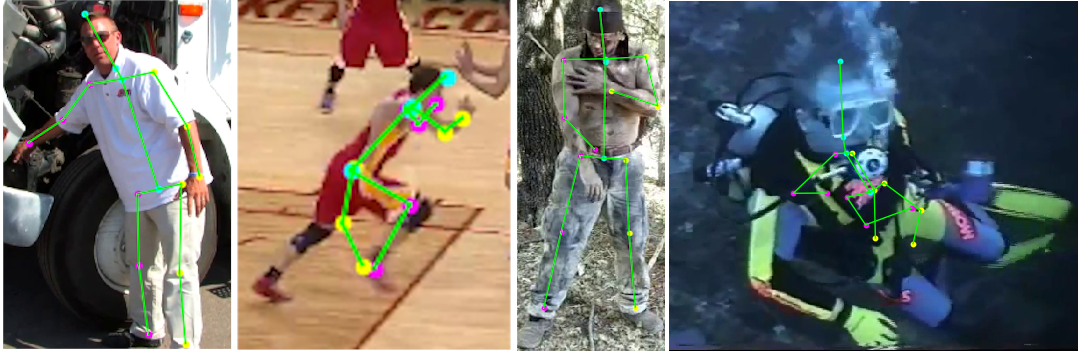
\includegraphics[width=0.99\textwidth]{mpii_example_results.png}
    \caption{Example images from the validation dataset after training a pose estimator using $8$ prediction blocks and using $2$ context heatmaps. The joints on the right side of the body (from the subjects perspective) are shown in magenta, while the joints on the left side are shown in yellow. The remaining joints are shown in cyan. \textbf{From left to right}: \textbf{1.} The pose estimator was able to estimate the ground truth pose correctly. \textbf{2.} The pose estimator confused right and left joints. Also, the estimator was not able to estimate the right ankle joint position correctly and wrongly estimated the joint position at the left ankle. \textbf{3.} The belt of the subject was wrongly estimated to be the right wrist. \textbf{4.} The pose estimator was not able to estimate the subjects pose, except for the head joint. This is most likely due to the fact that the subject is underwater and because the subject is wearing a diving suit.}
    \label{fig:mpii_example_results}
\end{figure}
In conclusion, while the test accuracy scores are significantly lower in comparison to the scores provided by the authors, this is most likely due to the difference in evaluation technique.
Moreover, there were no statistically significant differences found between the different model configurations, except for the difference between the $2$ and $8$ prediction block models.
Additionally, using context heatmaps does not significantly increase the accuracy of the pose estimator.

\subsubsection{HAR using Penn Action dataset}
To recreate the Human Activity Recognition results from \cite{luvizon_2d/3d_2018} on the Penn Action dataset, we first train a pose estimator.
Once the pose estimator is trained, its pretrained weights are used in the HAR model.
The authors used a hybrid dataset for training, consisting of $75\%$ MPII and of $25\%$ Penn Action training data.
They do not, however, motivate this decision.
The pose estimator contains $4$ prediction blocks, uses $2$ context heatmaps and it is trained using a batch size of $30$ and a learning rate of $10^{-3}$.
The validation accuracy scores achieved on the Penn Action validation dataset can be seen in \fref{fig:pose_mixed_results}.
% TODO: test on test dataset aswell
% TODO: Discuss results 

\begin{figure}[htb!]
    \centering
    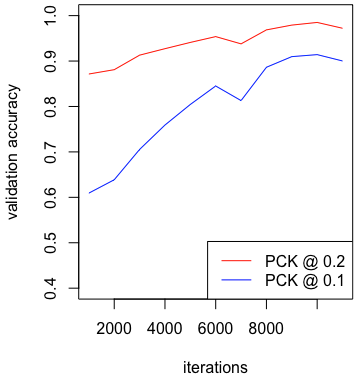
\includegraphics[width=0.45\textwidth]{pose_mixed_results.png}
    \caption{Validation accuracies computed during the training of the pose estimator. The training dataset is a mixture of $75\%$ MPII and $25\%$ Penn Action data. The validation accuracies are computed on the validation split of the Penn Action dataset. }
    \label{fig:pose_mixed_results}
\end{figure}

The pretrained pose estimator weights are inserted into the HAR model after the training process of the pose estimator finished.
The model is trained using Penn Action training data.
Also, the weights of the pose estimator are initially frozen.
The HAR model is then trained until the validation accuracies stops increasing, at which point the authors unfreeze the weights of the pose estimator and lower the learning rate.
The model is then fine-tuned in an end-to-end approach.
As an optimizer, the Stochastic Gradient Descend is used, with the addition of a momentum value $\gamma = 0.98$ and the use of a method called \textit{Nesterov Accelerated Gradient (NAG)} \cite{nesterov_method_1983}.

Momentum is used to accelarate the gradient descent process by incorporating a fraction $\gamma$ of the previous gradients when computing the new gradients.
Consider a regular update to the weights $w$ of a neuron using gradient descent, as explained in \sref{sec:gradient_descent}, given by

\begin{equation}
    w_{t+1} = w_t - \eta \nabla w_t,
\end{equation}

where $\eta$ refers to the learning rate and $\nabla w_t$ refers to the gradients w.r.t. $w_t$.
When using momentum, a update term $\nu_t$ is computed following

\begin{equation}
    \nu_t = \gamma \nu_{t-1} + \eta \nabla w_t.
\end{equation}

Afterwards, the new weights are computed by subtracting $\nu_t$ from $w_t$:

\begin{equation}
    w_{t+1} = w_t - \nu_t.
\end{equation}

The intuition behind momentum is that the descend towards the local minimum of the loss function can be accelerated by assuming that the gradients do not change significantly.
If gradients with a similar direction were multiple times before, then the assumption is that the next gradients will be similar as well.
This assumption, however, can lead to the case where the local minimum of the loss function is surpassed, which is often refered to as \textit{overshooting} the minimum.
To minimize the probability overshooting while still accelerating the descend towards the local minimum, Nesterov Accelerated Gradient adds an additional step to the momentum process.
It calculates a \textit{look-ahead} weight $w_{la} = w_{t} \gamma \nu_{t-1}$ and evaluates the gradient using this new weight.
If the gradient at $w_{la}$ points to a different direction than $\gamma \nu_{t-1}$ it will correct the surpassing of the minimum to an extend by reducing changing the direction of the gradient slighlty.
The following formula describes the update process of weights $w_t$ using the NAG:

\begin{equation}
    w_{t+1} = w_t - (\gamma \nu_{t-1} + \eta \nabla w_{la}).
\end{equation}

In the experiment conducted in this thesis, the validation does not increase after the TODO iteration
A learning rate of $2^{-5}$ is used, as suggested by the authors in their work.

\begin{figure}[htb!]
    \centering
    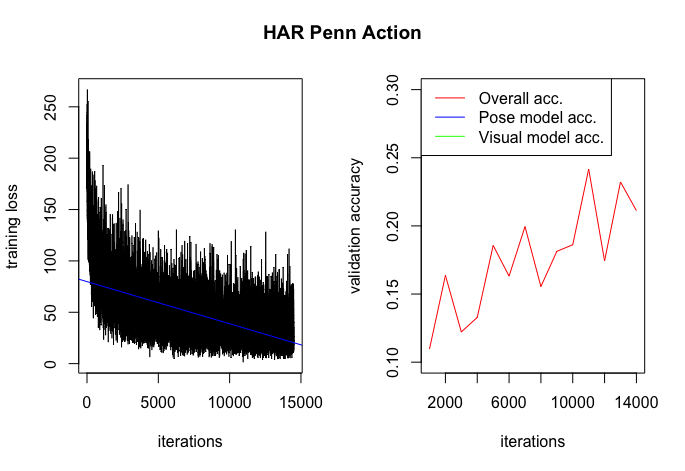
\includegraphics[width=0.8\textwidth]{har_pennaction_results.png}
    \caption{TODO}
    \label{fig:har_pennaction_results}
\end{figure}

- Started finetuning at iteration X and reduce learning rate by X % TODO
- Talk about results
% TODO: on test: confusion matrix for action and per-joint accuracy before and after finetuning. discuss changes
% TODO: show good / bad example images
% TODO: single and multi clip evaluation
% TODO: statistical significance testing between my results and authors
% TODO: zwischenfazit

\subsection{Pose estimation on JHMDB dataset}
\label{sec:exp-pose-jhmdb}
Similar to the experiment performed in \sref{sec:exp-replication}, this thesis evaluates different pose estimator configurations using the JHMDB dataset.
Specifically, pose estimators with $2, 4$ and $8$ prediction blocks are trained with and without context heatmaps to assess the performance of the network on a more challenging video dataset in terms of action diversity.
In terms of the pose estimator architecture, there are no changes to the experiments on the MPII dataset.

One assumption this thesis makes is that the ground truth bounding boxes for training, validation and test datasets are given.
This assumption was also made by \cite{luvizon_2d/3d_2018} for training and evaluating the pose estimator on the MPII dataset.
The accuracies, computed using three different metrics, are shown in \tref{tab:jhmdb_results}.
As can be seen, the best performing pose estimator configuration is $4$ prediction blocks and $0$ context heatmaps.
Notice that the test accuracies when using $8$ prediction blocks are significantly lower in comparison to the other configurations.
This is most likely due to the limited amount of data of the JHMDB dataset.
This hypothesis is supported by the fact that the accuracies when using context heatmaps are lower, in comparison to not using context heatmaps.
Context heatmaps introduce additional parameters to the pose estimator model, which need to be trained.
In general, the higher the number of parameters of a model, the more training data is needed to fit the model.

The $p$-values in \tref{tab:jhmdb_results} indicate that, for a pose estimator configuration with $2$ prediction blocks, adding context heatmaps significantly decreases the accuracy of the model.
This is most likely due to an increase in parameters of the pose estimator, which means that more data is necessary to fit the model.
This also applies to the configurations using $4$ prediction blocks, where the evaluated metrics are also lower when using context heatmaps.
These findings imply that the utility of context heatmaps is highly dependend on the training dataset size.
Interestingly, when using $8$ prediction blocks, the opposite appears to be true.
In \sref{sec:exp-mpii-pose}, it was found that the use of context heatmaps only significantly increased the accuracy of the pose estimator if $8$ prediction blocks were used.
This finding, in combination with the findings on the pose estimator trained on the JHMDB dataset, indicate that using context heatmaps only positively impacts the accuracy of a pose estimator if a high number of prediction blocks are used.
One reason for this might be that context heatmaps benefit from the refinement process of the stacked architecture more than the regular heatmaps (see \sref{sec:deephar_architecture}).  

\begin{table}[]
    \small
    \centering
    \begin{tabular}{|l|c|c|c||c|c|c||c|c|c|}
    \hline
        & & & \textbf{p-value} & & & \textbf{p-value} & & & \textbf{p-value} \\ \hline
        \textbf{nr\_blocks} & 2 & 2 &  & 4 & 4 &  & 8 & 8 &  \\ \hline
    \textbf{nr\_context} & 0 & 2 & & 0 & 2 & & 0 & 2 &\\ \hline
        \textbf{PCK @ 0.2} & 96.85 & 95.61 & \textbf{0.0} & \textbf{96.94} & 96.06 & \textbf{0.0} & 74.95 & 75.47 & 0.408 \\ \hline
        \textbf{PCK @ 0.1} & \textbf{92.03} & 90.20 & \textbf{0.0} & 91.69 & 90.95 & 0.072 & 50.13 & 52.14 & \textbf{0.005} \\ \hline
        \textbf{PCKu @ 0.2} & 87.32 & 86.21 & \textbf{0.031} & \textbf{87.49} & 86.92 &  0.224 & 44.03 & 45.30 & 0.085 \\ \hline
    \end{tabular}
    \caption{Test accuracies of the different pose estimator configurations, computed on the JHMDB test set. PCK is computed for two threshold values, $\alpha = 0.2$ as well as $\alpha = 0.1$. Additionally, PCKu is computed using $\alpha = 0.2$. Maximum values per metric, as well as $p$-values below the significance level of $0.05$, are shown in bold.}
    \label{tab:jhmdb_results}
\end{table}

In \tref{jhmdb_results_confidence}, the accuracies of different pose estimator configurations are compared using randomization testing.
The configurations with $8$ prediction blocks are ommited from this comparison, because their accuracies are much lower in comparison to the other configuration and there is no need for statistical significance testing.
It is found that there are no statistically significant differences between the accuracies of the tested configurations for any metric.
This is consistend with the findings in \sref{sec:exp-mpii-pose}, where the only significant differences were found between $8$ and $2$ prediction blocks.

\begin{table}[]
    \small
    \centering
    \begin{tabular}{|l|c|c|c||c|c|c|}
        \hline
            & & & \textbf{p-value} & & & \textbf{p-value} \\ \hline
            \textbf{nr\_blocks} & 2 & 4 &  & 2 & 4 &  \\ \hline
            \textbf{nr\_context} & 0 & 0 & & 2 & 2 & \\ \hline
            \textbf{PCK @ 0.2} & 96.85 & \textbf{96.94} & 0.689 & 95.61 & 96.06 & 0.121 \\ \hline
            \textbf{PCK @ 0.1} & \textbf{92.03} & 91.69 & 0.396 & 90.20 & 90.95 & 0.089 \\ \hline
            \textbf{PCKu @ 0.2} & 87.32 & \textbf{87.49} & 0.742 & 86.21 & 86.92 & 0.164 \\ \hline
        \end{tabular}
    \caption{Different model configurations for estimating pose on the JHMDB dataset, with their corresponding accuracy values. The configurations using $8$ prediction blocks are ommited because the results are significantly worse in comparion to the other configurations. The $p$-values were computed using a randomization test. None of the $p$-values are below the significance level of $0.05$.}
    \label{tab:jhmdb_results_confidence}
\end{table}

Next, the accuracy of best performing pose estimator configuration ($4$ prediction blocks, $0$ context heatmaps) with regards to individual joints and groupings of joints is evaluated in \tref{tab:jhmdb-perjoint}.
As a metric, PCK using $\alpha = 0.1$ is used, since this metric more precise in comparison to PCK using $\alpha = 0.2$, which aids in determining the differences between the individual joint accuracies.
In comparison to the joint accuracies computed in \tref{tab:mpii_test}, it becomes apparent that left and right ankles are more accurately estimated on the JHMDB dataset.
On both datasets, the joints associated with the head and torse region of the subject, i.e., upper neck, pelvis and head, are the most accurate.
One explaination for this is that there is less confusion with other, similar looking joints.
For example, while the left ankle might easily be confused with the right ankle, the head and torso region joints do not have a similarly looking counterpart.
In addition, these joints are less articulated, meaning that they do not change in position between different actions performed.

\begin{table}[]
    \small
    \centering
    \scalebox{0.90}{%
    \begin{tabular}{|c|c|c|c|c|c|c|c|}
    \hline
        \textbf{Ankle (r)} & \textbf{Knee (r)}  & \textbf{Hip (r)} & \textbf{Hip (l)} & \textbf{Knee (l)} & \textbf{Ankle (l)} & \textbf{Pelvis} & \textbf{Upper neck} \\ \hline
        0.87 & 0.84 & 0.90 & 0.88 & 0.83 & 0.85 & 0.93 & 0.94 \\ \hline \hline
        \textbf{Head top} & \textbf{Wrist (r)} & \textbf{Elbow (r)} & \textbf{Shoulder (r)} & \textbf{Shoulder (l)} & \textbf{Elbow (l)} & \textbf{Wrist (l)} & \textbf{Total} \\ \hline
        0.97 & 0.83  & 0.87 & 0.89 & 0.89 & 0.82 & 0.82 & 0.92 \\ \hline \hline
        \textbf{Arms (l)} & \textbf{Arms (r)} & \textbf{Arms (both)} & \textbf{Legs (l)} & \textbf{Legs (r)} & \textbf{Legs (both)} & \textbf{Upper body} & \textbf{Lower body}  \\ \hline
        0.84 & 0.86 & 0.85 & 0.85 & 0.87 & 0.86 & 0.88 & 0.87 \\ \hline
    \end{tabular}}
    \caption{Per joint accuracy w.r.t. PCK @ 0.1, computed on the JHMDB test set using $4$ prediction blocks and $0$ context heatmaps. In addition, aggregated accuracy values are given in the third row for different sets of joints. \textit{Arms} for both left and right are computed by taking the average of the shoulder, elbow and wrist accuracies. \textit{Legs} are computed the same way, using knee, ankle and hip accuracy values. For \textit{Upper body}, upper neck and head top are added to both \textit{Arms} aggregations. \textit{Lower body} is computed by aggregating both \textit{Legs} accuracies and pelvis accuracy.}
    \label{tab:jhmdb-perjoint}
\end{table}

As discussed before, this thesis assumed that human bounding boxes are given for training, validation and testing data.
When comparing our results to the state-of-the-art approach by \cite{song_thin-slicing_2017}, it was noted that our results outperforms the state-of-the-art.
The authors report a PCK accuracy of $81.6\%$ using $\alpha = 0.2$ and $68.7\%$ using $\alpha = 0.1$.
In comparison, our best performing model with $4$ prediction blocks and $0$ context heatmaps achieved $96.94\%$ PCK accuracy using $\alpha = 0.2$ and $91.69\%$ using $\alpha = 0.1$.
However, the authors of \cite{song_thin-slicing_2017} do not mention whether or not they used ground truth bounding boxes for the subject while training or evaluating their model.
Thus, it was decided to estimate the bounding box of the test data before estimating the pose using the approach outlined in TODO.
The results can be seen in \tref{tab:jhmdb_results_estimated}.
When comparing the results to \cite{song_thin-slicing_2017} using estimated bounding boxes on the test data, it becomes clear that our model is not able outperform the state-of-the-art.
% TODO: Explain estimation of bounding box in Penn Action HAR (since that is what the authors do)


\begin{table}[]
    \small
    \centering
    \begin{tabular}{|l|c|c|c|c|c|c|c|}
    \hline
         & & & & & & & \cite{song_thin-slicing_2017} \\ \hline
        \textbf{nr\_blocks} & 2 & 2 & 4 & 4 & 8 & 8 & -\\ \hline
        \textbf{nr\_context} & 0 & 2 & 0 & 2 & 0 & 2 & -\\ \hline
        \textbf{PCK @ 0.2} & 72.20 & \textbf{75.94} & 74.80 & 73.25 & 51.10 & 51.78 & 81.6 \\ \hline
        \textbf{PCK @ 0.1} & 41.53 & \textbf{45.77} & 43.82 & 41.76 & 20.82 & 21.42 & 68.70 \\ \hline
        \textbf{PCKu @ 0.2} & 33.77 & \textbf{38.02} & 35.47 & 34.55 & 19.22 & 19.81 & -\\ \hline
    \end{tabular}
    \caption{Test accuracies of the JHMDB pose estimation models when using estimated bounding boxes for the test data. In comparison to the state-of-the-art approach by \cite{song_thin-slicing_2017}, our model achieves notably lower accuracy values in both metrics. The highest accuracies achieved by our methods are shown in bold.}
    \label{tab:jhmdb_results_estimated}
\end{table}

In conclusion, pose estimation on the JHMDB dataset appears to be harder in comparison to the MPII dataset.
One reason might be the small size of the JHMDB dataset.
Also, since the JHMDB dataset is a video dataset, it contains video artifacts such as blur and camera jitter.
Moreover, the resolution of the frames is significantly lower in comparison to the MPII dataset.
This means that, since images from both dataset are resized to $256 \times 256$ pixels, the images from the JHMDB dataset contain more artifacts due to scaling and compression. 
% TODO: Conclusion chapter: mention that, for future work, higher resolution images are also ideal

\subsection{HAR on JHMDB Dataset}
To assess the performance of the action recognition model on the JHMDB dataset, the pretrained pose estimator with $4$ blocks and $2$ context maps from TODO is used, in order to compare the results to the performance on the Penn Action dataset experiment TODO.
The batch size is set to $12$ since the GPU used for experimentation did not allow for a bigger batch size.
Keep in mind that, since JHMDB is a video dataset, each item in the batch contains $16$ frames (see \sref{sec:exp-jhmdb}).
Effectively, this leads to a batch size of $16 \cdot batch\_size$ for the pose estimator since the pose for each frame is computed independently, before aggregating the estimated poses into the pose cube (see \sref{sec:pose_based_action_recognition}).
Similar to before, the point where the validation data accuracy does not increase further is found by training the model with a pose estimator whos weights are initially fixed.
As an initial learning rate, $2^{-5}$ is chosen, since this is the value used in the Penn Action HAR experiment.
Additionally, an augmentation ratio $1:6$ is used.

% TODO: reference the following image

\begin{figure}[htb!]
    \centering
    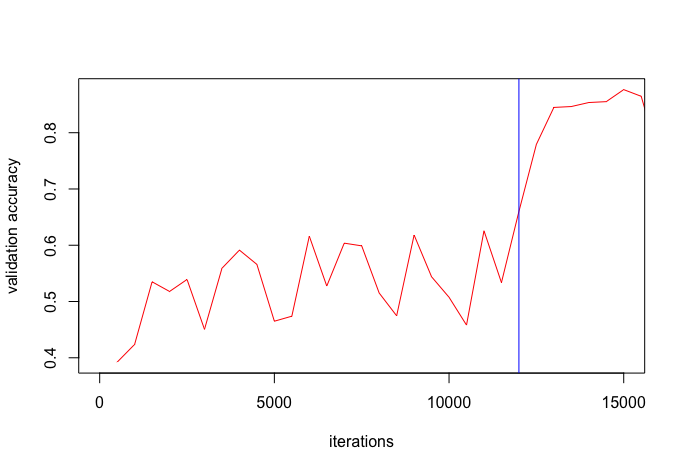
\includegraphics[width=0.8\textwidth]{har_jhmdb_combined.png}
    \caption{HAR JHMDB. TODO}
    \label{fig:har_jhmdb_combined}
\end{figure}

%bal

After approximately $15.000$ iterations, the validation accuracy plateaus.
At iteration $12.000$, the augmentation ratio is increased to $1:10$, and the learning rate is reduced to $10^{-6}$ since the model started overfitting.
Afterwards, the weights of the pose estimator are unfrozen and the finetuning process is started.
A smaller batch size of $2$ is used since the additional storage of computed gradients of the model inside the GPU virtual memory does not allow for a higher batch size.

% TODO: Validation without finetune: 82.81, 89.11 (single / multi)
% TODO: show validation and test accuracies
% TODO: on test: confusion matrix for action and per-joint accuracy before and after finetuning. discuss changes
% TODO: show good / bad example images
% TODO: Compare to PennAction
% TODO: We used gt bb because the model would not be able to achieve scores high enough

% TODO: Do graphic with all different experiments combined (validation). Until 12k: ares/no_finetune_with_td_aug6. Refine: kronos/no_finetune_with_td_refined_smaller_lr. Finetuning: kronos/with_finetune_with_td_refine start at 15k, batch size 2 because otherwise model does not fit because more gradients need to be stored in gpu memory.

\subsection{Effect of Combining Loss Functions}
Next, this thesis proposes a method for training the network in an end-to-end approach.
This means that no part of the network is pretrained.
To achieve this, the loss of the pose estimator and the loss of the action recognition pipeline are combined.
First, during the training process, the losses of all intermediate results from the pose estimator are computed using the elastic net loss.
Second, the loss of all intermediate results from the action recognition are computed using categorical cross-entropy.
It was decided to weigh both losses equally, i.e., sum them without weighting either the pose estimation or action recognition loss more in order to not make any assumptions about which part is more important.

The network needs a high amount of iterations for training until the validation accuracy converges.
This is to be expected, since no part of the network is pretrained and thus all parts have to be trained from random initialization.
See \fref{fig:e2e_big} for a graphical representation of the training process.
Training accuracy of the action recognition part of the network quickly increases and is above the training accuracy of the pose estimator in the beginning.  
This is to be expected since, at the beginning, the pose information is not reliable.
Thus, the network focuses on utilizing visual features for classification.
After approximately $25.000$ iterations, the pose training accuracy surpasses the action train accuracy and continues to converge towards $1$.

HAR validation is "jittery". this indicates uncertainty on unseen data. 


\begin{figure}[htb!]
    \centering
    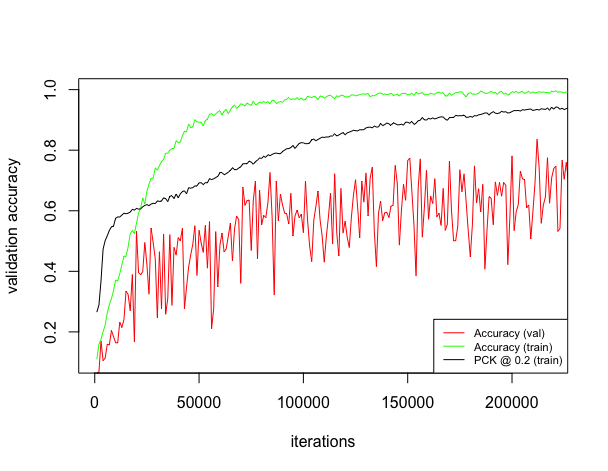
\includegraphics[width=0.8\textwidth]{e2e_big.png}
    \caption{Loss and validation accuracies of the pipeline trained using an end-to-end approach, without pretraining individual parts of the model. Validation accuracy given as percentage of correctly classified validation datapoints. TODO}
    \label{fig:e2e_big}
\end{figure}

\def \e2eFinalIteration {$228.000$ } % TODO

\begin{table}[]
    \small
    \centering
    \begin{tabular}{|c|c|c|c|c|}
    \hline
        \textbf{Single clip accuracy} & \textbf{Multi clip accuracy}  & \textbf{PCK @ 0.2} & \textbf{PCK @ 0.1} & \textbf{PCKu @ 0.2}\\ \hline
        0.81 & 0.84 & 0.83 & 0.51 & 0.36 \\ \hline
    \end{tabular}
    \caption{Test results on the JHMDB test set after \e2eFinalIteration iterations. TODO}
    \label{tab:e2e-quantitative-results}
\end{table}

% TODO: Compare action to pretrained
\tref{tab:e2e-quantitative-results}.
When comparing the pose accuracy of the end-to-end model to the pose estimators trained in \sref{sec:exp-pose-jhmdb}, it is apparent that the end-to-end model is significantly worse in all three metrics.
Further experimentation is necessary to assess whether or not the model hyperparameters like learning rate and batch size can be optimized in order for the end-to-end model to achieve comparable results to the pretrained model.
However, the findings are promising, because the network is , in general, able to achieve a high classification accuracy by being trained in an end-to-end approach.
This suggests that, while the pose estimator might be weaker in comparison to a standalone pose estimator, it is enough to make accurate action classifications.

\begin{figure}[htb!]
    \centering
    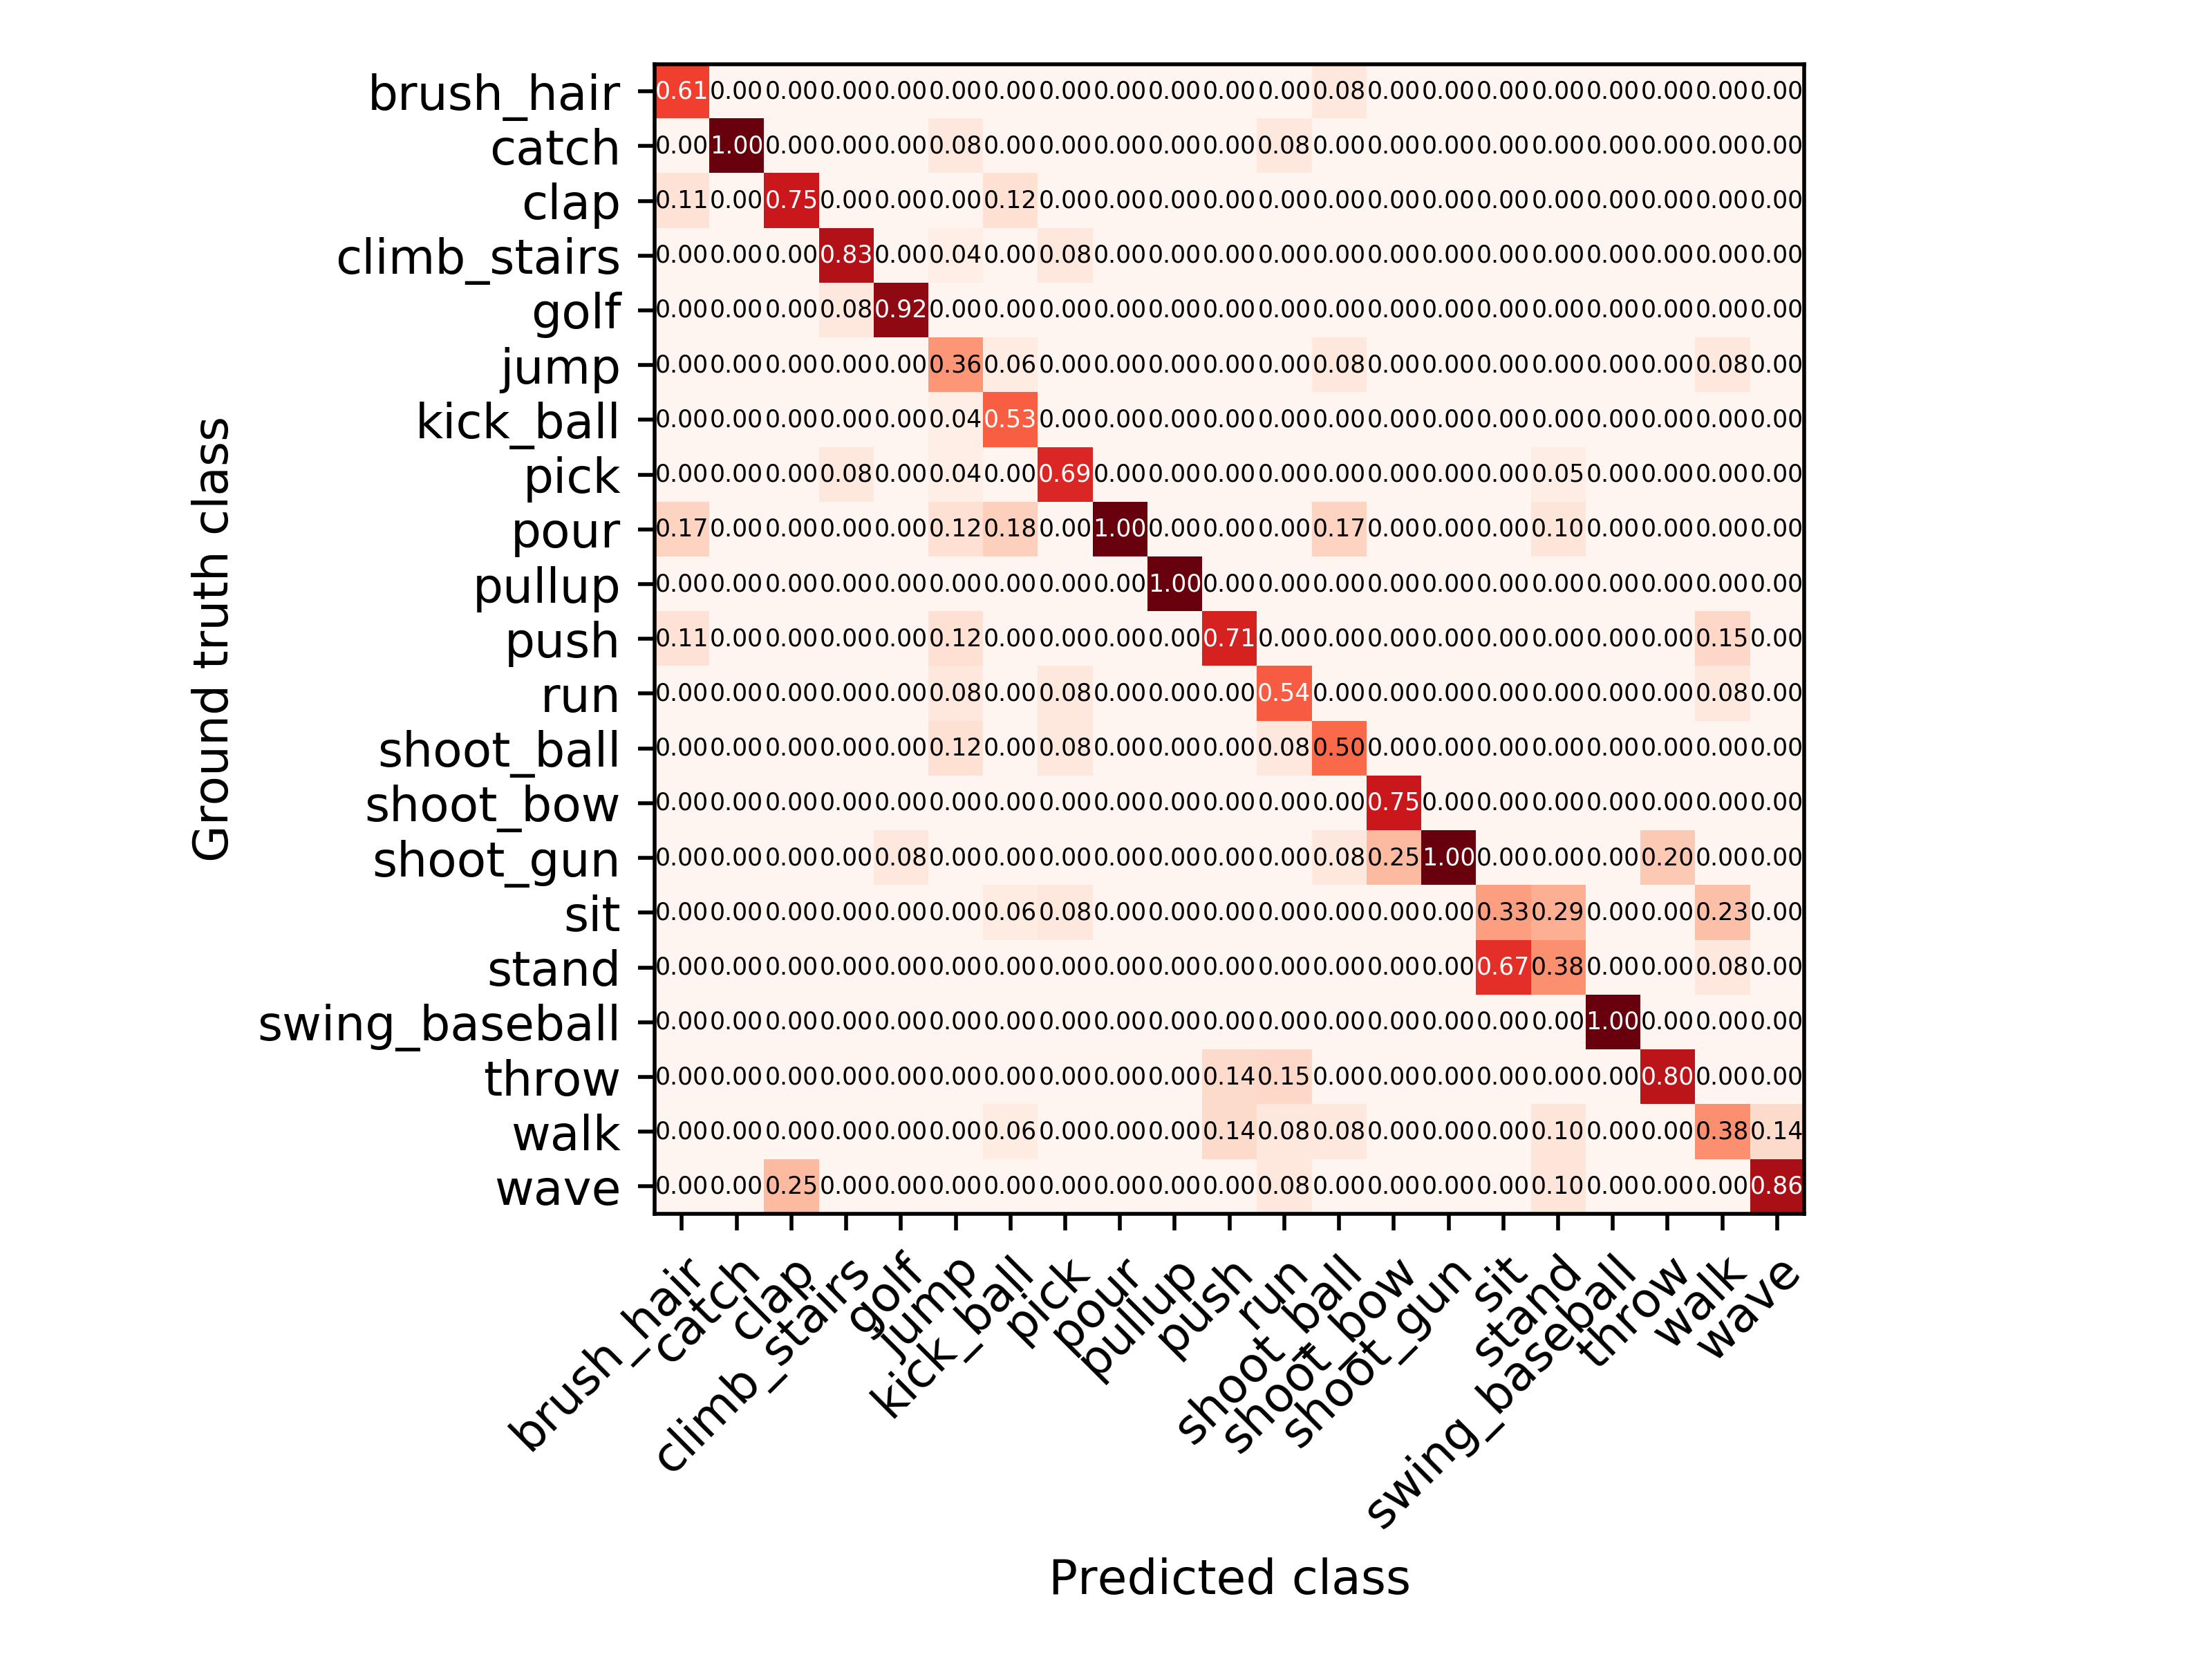
\includegraphics[width=0.999\textwidth]{cm-e2e.png}
    \caption{TODO}
    \label{fig:cm-e2e}
\end{figure}

A confusion matrix of the action classifcation on the test dataset is computed to gain a better understanding of the types of missclassification of the network (see \fref{fig:cm-e2e}).
From the confusion matrix, it becomes clear that the network is highly uncertain between the classes \textit{sit} and \textit{stand}.
Only $17\%$ of the test datapoints classified as \textit{stand} were actually from the \textit{stand} class.
In addition, in $39\%$ of the cases where the network predicted \textit{stand}, the ground truth class was \textit{sit}.

% TODO: Intraclass variance: half of each "sit" clip are people standing. see images for examples. Either classes in dataset need to be relabeled or network architecture needs to incorporate more temporal information because 16 frame chunks are not enough. future work!
% TODO: PUT THIS IN CONCLUSION CHAPTER

% One reason for such a large amount of confusion might be that the image context around the subject does not give a clear indication of the action, especially when considering the \textit{stand} class.
% Consider the high accuracy of the model on classes such as \textit{pullup} and \textit{golf}, where each image contains the object used in the interaction, in these cases a pullup bar and a golf club.
% This might also explain why the network is able to correctly estimate the \textit{sit} class in $83\%$ of test data, since a chair or other object the subject is sitting on might lead to useful image features.
% In addition, pose information of the upper body are very similar in both cases, which leads to another possible point of confusion.

% TODO: said stand, was wave
$22\%$ of test images are wrongly classified as \textit{stand}, when the actual class is \textit{wave}.
Would probably be better with more accurate pose at the hands.
Also intraclass variance

% TODO: show good / bad example images

% TODO: Comparison to JHMDB HAR with pretrained


\begin{table}[]
    \small
    \centering
    \scalebox{0.90}{%
    \begin{tabular}{|c|c|c|c|c|c|c|c|}
    \hline
        \textbf{Ankle (r)} & \textbf{Knee (r)}  & \textbf{Hip (r)} & \textbf{Hip (l)} & \textbf{Knee (l)} & \textbf{Ankle (l)} & \textbf{Pelvis} & \textbf{Upper neck} \\ \hline
        0.55 & 0.52 & 0.63 & 0.64 & 0.48 & 0.50 & 0.56 & 0.72 \\ \hline \hline
        \textbf{Head top} & \textbf{Wrist (r)} & \textbf{Elbow (r)} & \textbf{Shoulder (r)} & \textbf{Shoulder (l)} & \textbf{Elbow (l)} & \textbf{Wrist (l)} & \textbf{Total} \\ \hline
        0.75 & 0.31  & 0.37 & 0.47 & 0.54 & 0.45 & 0.47 & 0.51 \\ \hline \hline
        \textbf{Arms (l)} & \textbf{Arms (r)} & \textbf{Arms (both)} & \textbf{Legs (l)} & \textbf{Legs (r)} & \textbf{Legs (both)} & \textbf{Upper body} & \textbf{Lower body}  \\ \hline
        0.49 & 0.39 & 0.44 & 0.54 & 0.57 & 0.55 & 0.51 & 0.56 \\ \hline \hline
    \end{tabular}}
    \caption{Per joint accuracy, computed on the JHMDB test set using PCK @ 0.1 meassure. In addition, aggregated accuracy values are given in the third row for different sets of joints. \textit{Arms} for both left and right are computed by taking the average of the shoulder, elbow and wrist accuracies. \textit{Legs} are computed the same way, using knee, ankle and hip accuracy values. For \textit{Upper body}, upper neck and head top are added to both \textit{Arms} aggregations. \textit{Lower body} is computed by aggregating both \textit{legs} accuracies as well as pelvis.}
    \label{tab:e2e-perjoint}
\end{table}

In \tref{tab:e2e-perjoint}, the accuracy of the poses are given for each joint, as well as for some aggregations like \textit{upper body}.
On average, the network is more precise on the joints associated with the legs in comparison to the arm joints.
Also, joints associated with the right side of the subjects are detected with a higher accuracy than the joints associated with the left side.
% TODO: I think the same thing happens with JHMDB. Check and reference back!
% TODO: Why?

%TODO: explain why it didnt work (or why it did)
% TODO: Idea: show heatmaps per actions or joint accuracies per action. This would be better for explanation
